
% Default to the notebook output style

    


% Inherit from the specified cell style.




    
\documentclass[11pt]{article}

    
    
    \usepackage[T1]{fontenc}
    % Nicer default font (+ math font) than Computer Modern for most use cases
    \usepackage{mathpazo}

    % Basic figure setup, for now with no caption control since it's done
    % automatically by Pandoc (which extracts ![](path) syntax from Markdown).
    \usepackage{graphicx}
    % We will generate all images so they have a width \maxwidth. This means
    % that they will get their normal width if they fit onto the page, but
    % are scaled down if they would overflow the margins.
    \makeatletter
    \def\maxwidth{\ifdim\Gin@nat@width>\linewidth\linewidth
    \else\Gin@nat@width\fi}
    \makeatother
    \let\Oldincludegraphics\includegraphics
    % Set max figure width to be 80% of text width, for now hardcoded.
    \renewcommand{\includegraphics}[1]{\Oldincludegraphics[width=.8\maxwidth]{#1}}
    % Ensure that by default, figures have no caption (until we provide a
    % proper Figure object with a Caption API and a way to capture that
    % in the conversion process - todo).
    \usepackage{caption}
    \DeclareCaptionLabelFormat{nolabel}{}
    \captionsetup{labelformat=nolabel}

    \usepackage{adjustbox} % Used to constrain images to a maximum size 
    \usepackage{xcolor} % Allow colors to be defined
    \usepackage{enumerate} % Needed for markdown enumerations to work
    \usepackage{geometry} % Used to adjust the document margins
    \usepackage{amsmath} % Equations
    \usepackage{amssymb} % Equations
    \usepackage{textcomp} % defines textquotesingle
    % Hack from http://tex.stackexchange.com/a/47451/13684:
    \AtBeginDocument{%
        \def\PYZsq{\textquotesingle}% Upright quotes in Pygmentized code
    }
    \usepackage{upquote} % Upright quotes for verbatim code
    \usepackage{eurosym} % defines \euro
    \usepackage[mathletters]{ucs} % Extended unicode (utf-8) support
    \usepackage[utf8x]{inputenc} % Allow utf-8 characters in the tex document
    \usepackage{fancyvrb} % verbatim replacement that allows latex
    \usepackage{grffile} % extends the file name processing of package graphics 
                         % to support a larger range 
    % The hyperref package gives us a pdf with properly built
    % internal navigation ('pdf bookmarks' for the table of contents,
    % internal cross-reference links, web links for URLs, etc.)
    \usepackage{hyperref}
    \usepackage{longtable} % longtable support required by pandoc >1.10
    \usepackage{booktabs}  % table support for pandoc > 1.12.2
    \usepackage[inline]{enumitem} % IRkernel/repr support (it uses the enumerate* environment)
    \usepackage[normalem]{ulem} % ulem is needed to support strikethroughs (\sout)
                                % normalem makes italics be italics, not underlines
    

    
    
    % Colors for the hyperref package
    \definecolor{urlcolor}{rgb}{0,.145,.698}
    \definecolor{linkcolor}{rgb}{.71,0.21,0.01}
    \definecolor{citecolor}{rgb}{.12,.54,.11}

    % ANSI colors
    \definecolor{ansi-black}{HTML}{3E424D}
    \definecolor{ansi-black-intense}{HTML}{282C36}
    \definecolor{ansi-red}{HTML}{E75C58}
    \definecolor{ansi-red-intense}{HTML}{B22B31}
    \definecolor{ansi-green}{HTML}{00A250}
    \definecolor{ansi-green-intense}{HTML}{007427}
    \definecolor{ansi-yellow}{HTML}{DDB62B}
    \definecolor{ansi-yellow-intense}{HTML}{B27D12}
    \definecolor{ansi-blue}{HTML}{208FFB}
    \definecolor{ansi-blue-intense}{HTML}{0065CA}
    \definecolor{ansi-magenta}{HTML}{D160C4}
    \definecolor{ansi-magenta-intense}{HTML}{A03196}
    \definecolor{ansi-cyan}{HTML}{60C6C8}
    \definecolor{ansi-cyan-intense}{HTML}{258F8F}
    \definecolor{ansi-white}{HTML}{C5C1B4}
    \definecolor{ansi-white-intense}{HTML}{A1A6B2}

    % commands and environments needed by pandoc snippets
    % extracted from the output of `pandoc -s`
    \providecommand{\tightlist}{%
      \setlength{\itemsep}{0pt}\setlength{\parskip}{0pt}}
    \DefineVerbatimEnvironment{Highlighting}{Verbatim}{commandchars=\\\{\}}
    % Add ',fontsize=\small' for more characters per line
    \newenvironment{Shaded}{}{}
    \newcommand{\KeywordTok}[1]{\textcolor[rgb]{0.00,0.44,0.13}{\textbf{{#1}}}}
    \newcommand{\DataTypeTok}[1]{\textcolor[rgb]{0.56,0.13,0.00}{{#1}}}
    \newcommand{\DecValTok}[1]{\textcolor[rgb]{0.25,0.63,0.44}{{#1}}}
    \newcommand{\BaseNTok}[1]{\textcolor[rgb]{0.25,0.63,0.44}{{#1}}}
    \newcommand{\FloatTok}[1]{\textcolor[rgb]{0.25,0.63,0.44}{{#1}}}
    \newcommand{\CharTok}[1]{\textcolor[rgb]{0.25,0.44,0.63}{{#1}}}
    \newcommand{\StringTok}[1]{\textcolor[rgb]{0.25,0.44,0.63}{{#1}}}
    \newcommand{\CommentTok}[1]{\textcolor[rgb]{0.38,0.63,0.69}{\textit{{#1}}}}
    \newcommand{\OtherTok}[1]{\textcolor[rgb]{0.00,0.44,0.13}{{#1}}}
    \newcommand{\AlertTok}[1]{\textcolor[rgb]{1.00,0.00,0.00}{\textbf{{#1}}}}
    \newcommand{\FunctionTok}[1]{\textcolor[rgb]{0.02,0.16,0.49}{{#1}}}
    \newcommand{\RegionMarkerTok}[1]{{#1}}
    \newcommand{\ErrorTok}[1]{\textcolor[rgb]{1.00,0.00,0.00}{\textbf{{#1}}}}
    \newcommand{\NormalTok}[1]{{#1}}
    
    % Additional commands for more recent versions of Pandoc
    \newcommand{\ConstantTok}[1]{\textcolor[rgb]{0.53,0.00,0.00}{{#1}}}
    \newcommand{\SpecialCharTok}[1]{\textcolor[rgb]{0.25,0.44,0.63}{{#1}}}
    \newcommand{\VerbatimStringTok}[1]{\textcolor[rgb]{0.25,0.44,0.63}{{#1}}}
    \newcommand{\SpecialStringTok}[1]{\textcolor[rgb]{0.73,0.40,0.53}{{#1}}}
    \newcommand{\ImportTok}[1]{{#1}}
    \newcommand{\DocumentationTok}[1]{\textcolor[rgb]{0.73,0.13,0.13}{\textit{{#1}}}}
    \newcommand{\AnnotationTok}[1]{\textcolor[rgb]{0.38,0.63,0.69}{\textbf{\textit{{#1}}}}}
    \newcommand{\CommentVarTok}[1]{\textcolor[rgb]{0.38,0.63,0.69}{\textbf{\textit{{#1}}}}}
    \newcommand{\VariableTok}[1]{\textcolor[rgb]{0.10,0.09,0.49}{{#1}}}
    \newcommand{\ControlFlowTok}[1]{\textcolor[rgb]{0.00,0.44,0.13}{\textbf{{#1}}}}
    \newcommand{\OperatorTok}[1]{\textcolor[rgb]{0.40,0.40,0.40}{{#1}}}
    \newcommand{\BuiltInTok}[1]{{#1}}
    \newcommand{\ExtensionTok}[1]{{#1}}
    \newcommand{\PreprocessorTok}[1]{\textcolor[rgb]{0.74,0.48,0.00}{{#1}}}
    \newcommand{\AttributeTok}[1]{\textcolor[rgb]{0.49,0.56,0.16}{{#1}}}
    \newcommand{\InformationTok}[1]{\textcolor[rgb]{0.38,0.63,0.69}{\textbf{\textit{{#1}}}}}
    \newcommand{\WarningTok}[1]{\textcolor[rgb]{0.38,0.63,0.69}{\textbf{\textit{{#1}}}}}
    
    
    % Define a nice break command that doesn't care if a line doesn't already
    % exist.
    \def\br{\hspace*{\fill} \\* }
    % Math Jax compatability definitions
    \def\gt{>}
    \def\lt{<}
    % Document parameters
    \title{Project\_3}
    
    
    

    % Pygments definitions
    
\makeatletter
\def\PY@reset{\let\PY@it=\relax \let\PY@bf=\relax%
    \let\PY@ul=\relax \let\PY@tc=\relax%
    \let\PY@bc=\relax \let\PY@ff=\relax}
\def\PY@tok#1{\csname PY@tok@#1\endcsname}
\def\PY@toks#1+{\ifx\relax#1\empty\else%
    \PY@tok{#1}\expandafter\PY@toks\fi}
\def\PY@do#1{\PY@bc{\PY@tc{\PY@ul{%
    \PY@it{\PY@bf{\PY@ff{#1}}}}}}}
\def\PY#1#2{\PY@reset\PY@toks#1+\relax+\PY@do{#2}}

\expandafter\def\csname PY@tok@w\endcsname{\def\PY@tc##1{\textcolor[rgb]{0.73,0.73,0.73}{##1}}}
\expandafter\def\csname PY@tok@c\endcsname{\let\PY@it=\textit\def\PY@tc##1{\textcolor[rgb]{0.25,0.50,0.50}{##1}}}
\expandafter\def\csname PY@tok@cp\endcsname{\def\PY@tc##1{\textcolor[rgb]{0.74,0.48,0.00}{##1}}}
\expandafter\def\csname PY@tok@k\endcsname{\let\PY@bf=\textbf\def\PY@tc##1{\textcolor[rgb]{0.00,0.50,0.00}{##1}}}
\expandafter\def\csname PY@tok@kp\endcsname{\def\PY@tc##1{\textcolor[rgb]{0.00,0.50,0.00}{##1}}}
\expandafter\def\csname PY@tok@kt\endcsname{\def\PY@tc##1{\textcolor[rgb]{0.69,0.00,0.25}{##1}}}
\expandafter\def\csname PY@tok@o\endcsname{\def\PY@tc##1{\textcolor[rgb]{0.40,0.40,0.40}{##1}}}
\expandafter\def\csname PY@tok@ow\endcsname{\let\PY@bf=\textbf\def\PY@tc##1{\textcolor[rgb]{0.67,0.13,1.00}{##1}}}
\expandafter\def\csname PY@tok@nb\endcsname{\def\PY@tc##1{\textcolor[rgb]{0.00,0.50,0.00}{##1}}}
\expandafter\def\csname PY@tok@nf\endcsname{\def\PY@tc##1{\textcolor[rgb]{0.00,0.00,1.00}{##1}}}
\expandafter\def\csname PY@tok@nc\endcsname{\let\PY@bf=\textbf\def\PY@tc##1{\textcolor[rgb]{0.00,0.00,1.00}{##1}}}
\expandafter\def\csname PY@tok@nn\endcsname{\let\PY@bf=\textbf\def\PY@tc##1{\textcolor[rgb]{0.00,0.00,1.00}{##1}}}
\expandafter\def\csname PY@tok@ne\endcsname{\let\PY@bf=\textbf\def\PY@tc##1{\textcolor[rgb]{0.82,0.25,0.23}{##1}}}
\expandafter\def\csname PY@tok@nv\endcsname{\def\PY@tc##1{\textcolor[rgb]{0.10,0.09,0.49}{##1}}}
\expandafter\def\csname PY@tok@no\endcsname{\def\PY@tc##1{\textcolor[rgb]{0.53,0.00,0.00}{##1}}}
\expandafter\def\csname PY@tok@nl\endcsname{\def\PY@tc##1{\textcolor[rgb]{0.63,0.63,0.00}{##1}}}
\expandafter\def\csname PY@tok@ni\endcsname{\let\PY@bf=\textbf\def\PY@tc##1{\textcolor[rgb]{0.60,0.60,0.60}{##1}}}
\expandafter\def\csname PY@tok@na\endcsname{\def\PY@tc##1{\textcolor[rgb]{0.49,0.56,0.16}{##1}}}
\expandafter\def\csname PY@tok@nt\endcsname{\let\PY@bf=\textbf\def\PY@tc##1{\textcolor[rgb]{0.00,0.50,0.00}{##1}}}
\expandafter\def\csname PY@tok@nd\endcsname{\def\PY@tc##1{\textcolor[rgb]{0.67,0.13,1.00}{##1}}}
\expandafter\def\csname PY@tok@s\endcsname{\def\PY@tc##1{\textcolor[rgb]{0.73,0.13,0.13}{##1}}}
\expandafter\def\csname PY@tok@sd\endcsname{\let\PY@it=\textit\def\PY@tc##1{\textcolor[rgb]{0.73,0.13,0.13}{##1}}}
\expandafter\def\csname PY@tok@si\endcsname{\let\PY@bf=\textbf\def\PY@tc##1{\textcolor[rgb]{0.73,0.40,0.53}{##1}}}
\expandafter\def\csname PY@tok@se\endcsname{\let\PY@bf=\textbf\def\PY@tc##1{\textcolor[rgb]{0.73,0.40,0.13}{##1}}}
\expandafter\def\csname PY@tok@sr\endcsname{\def\PY@tc##1{\textcolor[rgb]{0.73,0.40,0.53}{##1}}}
\expandafter\def\csname PY@tok@ss\endcsname{\def\PY@tc##1{\textcolor[rgb]{0.10,0.09,0.49}{##1}}}
\expandafter\def\csname PY@tok@sx\endcsname{\def\PY@tc##1{\textcolor[rgb]{0.00,0.50,0.00}{##1}}}
\expandafter\def\csname PY@tok@m\endcsname{\def\PY@tc##1{\textcolor[rgb]{0.40,0.40,0.40}{##1}}}
\expandafter\def\csname PY@tok@gh\endcsname{\let\PY@bf=\textbf\def\PY@tc##1{\textcolor[rgb]{0.00,0.00,0.50}{##1}}}
\expandafter\def\csname PY@tok@gu\endcsname{\let\PY@bf=\textbf\def\PY@tc##1{\textcolor[rgb]{0.50,0.00,0.50}{##1}}}
\expandafter\def\csname PY@tok@gd\endcsname{\def\PY@tc##1{\textcolor[rgb]{0.63,0.00,0.00}{##1}}}
\expandafter\def\csname PY@tok@gi\endcsname{\def\PY@tc##1{\textcolor[rgb]{0.00,0.63,0.00}{##1}}}
\expandafter\def\csname PY@tok@gr\endcsname{\def\PY@tc##1{\textcolor[rgb]{1.00,0.00,0.00}{##1}}}
\expandafter\def\csname PY@tok@ge\endcsname{\let\PY@it=\textit}
\expandafter\def\csname PY@tok@gs\endcsname{\let\PY@bf=\textbf}
\expandafter\def\csname PY@tok@gp\endcsname{\let\PY@bf=\textbf\def\PY@tc##1{\textcolor[rgb]{0.00,0.00,0.50}{##1}}}
\expandafter\def\csname PY@tok@go\endcsname{\def\PY@tc##1{\textcolor[rgb]{0.53,0.53,0.53}{##1}}}
\expandafter\def\csname PY@tok@gt\endcsname{\def\PY@tc##1{\textcolor[rgb]{0.00,0.27,0.87}{##1}}}
\expandafter\def\csname PY@tok@err\endcsname{\def\PY@bc##1{\setlength{\fboxsep}{0pt}\fcolorbox[rgb]{1.00,0.00,0.00}{1,1,1}{\strut ##1}}}
\expandafter\def\csname PY@tok@kc\endcsname{\let\PY@bf=\textbf\def\PY@tc##1{\textcolor[rgb]{0.00,0.50,0.00}{##1}}}
\expandafter\def\csname PY@tok@kd\endcsname{\let\PY@bf=\textbf\def\PY@tc##1{\textcolor[rgb]{0.00,0.50,0.00}{##1}}}
\expandafter\def\csname PY@tok@kn\endcsname{\let\PY@bf=\textbf\def\PY@tc##1{\textcolor[rgb]{0.00,0.50,0.00}{##1}}}
\expandafter\def\csname PY@tok@kr\endcsname{\let\PY@bf=\textbf\def\PY@tc##1{\textcolor[rgb]{0.00,0.50,0.00}{##1}}}
\expandafter\def\csname PY@tok@bp\endcsname{\def\PY@tc##1{\textcolor[rgb]{0.00,0.50,0.00}{##1}}}
\expandafter\def\csname PY@tok@fm\endcsname{\def\PY@tc##1{\textcolor[rgb]{0.00,0.00,1.00}{##1}}}
\expandafter\def\csname PY@tok@vc\endcsname{\def\PY@tc##1{\textcolor[rgb]{0.10,0.09,0.49}{##1}}}
\expandafter\def\csname PY@tok@vg\endcsname{\def\PY@tc##1{\textcolor[rgb]{0.10,0.09,0.49}{##1}}}
\expandafter\def\csname PY@tok@vi\endcsname{\def\PY@tc##1{\textcolor[rgb]{0.10,0.09,0.49}{##1}}}
\expandafter\def\csname PY@tok@vm\endcsname{\def\PY@tc##1{\textcolor[rgb]{0.10,0.09,0.49}{##1}}}
\expandafter\def\csname PY@tok@sa\endcsname{\def\PY@tc##1{\textcolor[rgb]{0.73,0.13,0.13}{##1}}}
\expandafter\def\csname PY@tok@sb\endcsname{\def\PY@tc##1{\textcolor[rgb]{0.73,0.13,0.13}{##1}}}
\expandafter\def\csname PY@tok@sc\endcsname{\def\PY@tc##1{\textcolor[rgb]{0.73,0.13,0.13}{##1}}}
\expandafter\def\csname PY@tok@dl\endcsname{\def\PY@tc##1{\textcolor[rgb]{0.73,0.13,0.13}{##1}}}
\expandafter\def\csname PY@tok@s2\endcsname{\def\PY@tc##1{\textcolor[rgb]{0.73,0.13,0.13}{##1}}}
\expandafter\def\csname PY@tok@sh\endcsname{\def\PY@tc##1{\textcolor[rgb]{0.73,0.13,0.13}{##1}}}
\expandafter\def\csname PY@tok@s1\endcsname{\def\PY@tc##1{\textcolor[rgb]{0.73,0.13,0.13}{##1}}}
\expandafter\def\csname PY@tok@mb\endcsname{\def\PY@tc##1{\textcolor[rgb]{0.40,0.40,0.40}{##1}}}
\expandafter\def\csname PY@tok@mf\endcsname{\def\PY@tc##1{\textcolor[rgb]{0.40,0.40,0.40}{##1}}}
\expandafter\def\csname PY@tok@mh\endcsname{\def\PY@tc##1{\textcolor[rgb]{0.40,0.40,0.40}{##1}}}
\expandafter\def\csname PY@tok@mi\endcsname{\def\PY@tc##1{\textcolor[rgb]{0.40,0.40,0.40}{##1}}}
\expandafter\def\csname PY@tok@il\endcsname{\def\PY@tc##1{\textcolor[rgb]{0.40,0.40,0.40}{##1}}}
\expandafter\def\csname PY@tok@mo\endcsname{\def\PY@tc##1{\textcolor[rgb]{0.40,0.40,0.40}{##1}}}
\expandafter\def\csname PY@tok@ch\endcsname{\let\PY@it=\textit\def\PY@tc##1{\textcolor[rgb]{0.25,0.50,0.50}{##1}}}
\expandafter\def\csname PY@tok@cm\endcsname{\let\PY@it=\textit\def\PY@tc##1{\textcolor[rgb]{0.25,0.50,0.50}{##1}}}
\expandafter\def\csname PY@tok@cpf\endcsname{\let\PY@it=\textit\def\PY@tc##1{\textcolor[rgb]{0.25,0.50,0.50}{##1}}}
\expandafter\def\csname PY@tok@c1\endcsname{\let\PY@it=\textit\def\PY@tc##1{\textcolor[rgb]{0.25,0.50,0.50}{##1}}}
\expandafter\def\csname PY@tok@cs\endcsname{\let\PY@it=\textit\def\PY@tc##1{\textcolor[rgb]{0.25,0.50,0.50}{##1}}}

\def\PYZbs{\char`\\}
\def\PYZus{\char`\_}
\def\PYZob{\char`\{}
\def\PYZcb{\char`\}}
\def\PYZca{\char`\^}
\def\PYZam{\char`\&}
\def\PYZlt{\char`\<}
\def\PYZgt{\char`\>}
\def\PYZsh{\char`\#}
\def\PYZpc{\char`\%}
\def\PYZdl{\char`\$}
\def\PYZhy{\char`\-}
\def\PYZsq{\char`\'}
\def\PYZdq{\char`\"}
\def\PYZti{\char`\~}
% for compatibility with earlier versions
\def\PYZat{@}
\def\PYZlb{[}
\def\PYZrb{]}
\makeatother


    % Exact colors from NB
    \definecolor{incolor}{rgb}{0.0, 0.0, 0.5}
    \definecolor{outcolor}{rgb}{0.545, 0.0, 0.0}



    
    % Prevent overflowing lines due to hard-to-break entities
    \sloppy 
    % Setup hyperref package
    \hypersetup{
      breaklinks=true,  % so long urls are correctly broken across lines
      colorlinks=true,
      urlcolor=urlcolor,
      linkcolor=linkcolor,
      citecolor=citecolor,
      }
    % Slightly bigger margins than the latex defaults
    
    \geometry{verbose,tmargin=1in,bmargin=1in,lmargin=1in,rmargin=1in}
    
    

    \begin{document}
    
    
    \maketitle
    
    

    
    \hypertarget{project-3}{%
\section{Project 3}\label{project-3}}

Griffith Stites and Alex Hindelang

    \hypertarget{question-how-does-the-fluid-in-which-a-penguin-swims-change-its-maximum-velocity-and-swim-time}{%
\section{Question: How does the fluid in which a penguin swims change
its maximum velocity and swim
time?}\label{question-how-does-the-fluid-in-which-a-penguin-swims-change-its-maximum-velocity-and-swim-time}}

    We are modeling the motion of a penguin in olympic-sized swimming pool
filled with different fluids to test how its motion is affected.

    \begin{Verbatim}[commandchars=\\\{\}]
{\color{incolor}In [{\color{incolor}1}]:} \PY{c+c1}{\PYZsh{} Configure Jupyter so figures appear in the notebook}
        \PY{o}{\PYZpc{}}\PY{k}{matplotlib} inline
        
        \PY{c+c1}{\PYZsh{} Configure Jupyter to display the assigned value after an assignment}
        \PY{o}{\PYZpc{}}\PY{k}{config} InteractiveShell.ast\PYZus{}node\PYZus{}interactivity=\PYZsq{}last\PYZus{}expr\PYZus{}or\PYZus{}assign\PYZsq{}
        
        \PY{c+c1}{\PYZsh{} import functions from the modsim.py module}
        \PY{k+kn}{from} \PY{n+nn}{modsim} \PY{k}{import} \PY{o}{*}
        
        \PY{c+c1}{\PYZsh{} import matlab like plotting functions}
        \PY{k+kn}{import} \PY{n+nn}{matplotlib}
        \PY{k+kn}{import} \PY{n+nn}{matplotlib}\PY{n+nn}{.}\PY{n+nn}{pyplot} \PY{k}{as} \PY{n+nn}{plt}
        \PY{k+kn}{import} \PY{n+nn}{matplotlib}\PY{n+nn}{.}\PY{n+nn}{patches} \PY{k}{as} \PY{n+nn}{mpatches}
        \PY{k+kn}{from} \PY{n+nn}{matplotlib}\PY{n+nn}{.}\PY{n+nn}{pyplot} \PY{k}{import} \PY{n}{figure}
        \PY{k+kn}{from} \PY{n+nn}{scipy} \PY{k}{import} \PY{n}{signal}
        \PY{k+kn}{import} \PY{n+nn}{math}
\end{Verbatim}


    \hypertarget{model}{%
\section{Model}\label{model}}

    \hypertarget{assumptions}{%
\subsubsection{Assumptions}\label{assumptions}}

\begin{itemize}
\tightlist
\item
  Temperature changes for the fluid do not significantly change density.
  We choose based off of the listed temperature from the
  \href{https://www.engineeringtoolbox.com/liquids-densities-d_743.html}{Engineering
  Toolbox Chart}.
\item
  The force the penguin exerts on the fluid does not change based on
  fluid density. We made this assumption because it makes sense that
  there is a maximum force the penguin can exert regardless of density.
  For example, if it was pushing against an infinitely dense solid it
  could not exert an infinite force. However, it also makes sense that
  there would be a fluid that was not dense enough to exert maximum
  force onto it (like air). We chose to ignore this because although we
  have fluids heavier and lighter than sea water, they are not at either
  extreme.
\item
  Penguins flap their flippers 50\% of the time when exerting maximum
  force.
\item
  When penguins reset their flippers back to the ready to propel
  positions, they do not push themselves backwards at all. This
  assumption was made because we figured the force would be relatively
  small as penguins are efficient and aerodynamic swimmers.
\end{itemize}

    \hypertarget{schematic-diagram}{%
\subsubsection{Schematic Diagram}\label{schematic-diagram}}

    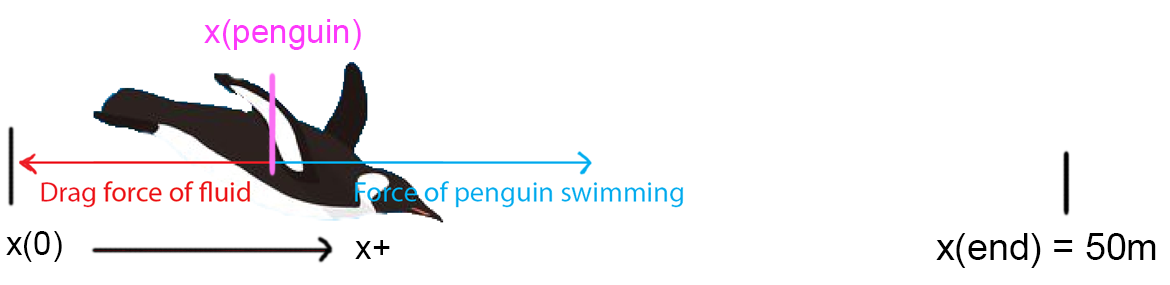
\includegraphics{https://raw.githubusercontent.com/ahindelang/ModSimPy/master/code/Untitled-1.png}

This is a 1-dimensional model, so the penguin only moves in the positive
x direction. The drag force is opposite to this. The simulation ends
when the penguin reaches the other side of an Olympic swimming pool,
which is 50 meters long.

    \hypertarget{differential-equations}{%
\subsubsection{Differential Equations}\label{differential-equations}}

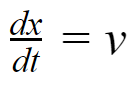
\includegraphics{https://raw.githubusercontent.com/ahindelang/ModSimPy/master/dx.PNG}

The change in distance over time is simply the velocity. The slope
function calculates the velocity using a separate differential equation.

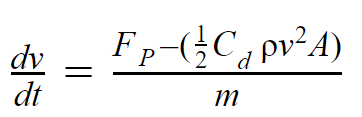
\includegraphics{https://raw.githubusercontent.com/ahindelang/ModSimPy/master/dv.PNG}

Fp refers to the force of the penguin. The term in parentheses is the
drag equation: Cd is the coefficient of drag, rho is the fluid density,
v is the velocity, and A is the reference area. The difference between
these two is the total force propelling the penguin forward. This is
divided by m (mass of the penguin) to find acceleration according to
Newton's 2nd Law of Motion.

    Our model uses force equations to derive the velocity and distance
traveled of a penguin. It runs a simulation of the force of the penguin
swimming versus the drag force and records the time it takes for the
penguin to travel the length of an Olympic swimming pool.

    \begin{Verbatim}[commandchars=\\\{\}]
{\color{incolor}In [{\color{incolor} }]:} \PY{n}{m} \PY{o}{=} \PY{n}{UNITS}\PY{o}{.}\PY{n}{meter}
        \PY{n}{s} \PY{o}{=} \PY{n}{UNITS}\PY{o}{.}\PY{n}{second}
        \PY{n}{kg} \PY{o}{=} \PY{n}{UNITS}\PY{o}{.}\PY{n}{kilogram}
        \PY{n}{km} \PY{o}{=} \PY{n}{UNITS}\PY{o}{.}\PY{n}{kilometer}
        \PY{n}{hr} \PY{o}{=} \PY{n}{UNITS}\PY{o}{.}\PY{n}{hour}
        \PY{n}{s} \PY{o}{=} \PY{n}{UNITS}\PY{o}{.}\PY{n}{second}
        \PY{n}{N} \PY{o}{=} \PY{n}{UNITS}\PY{o}{.}\PY{n}{newton}
        \PY{p}{;}
\end{Verbatim}


    We declared the values of different liquid densities: sea water, syrup,
and propyl alcohol. Sea water was chosen as it is the natural fluid of a
penguin and can be used as a control. It is also necessary for finding
the force of a penguin based on the max speed since max speed for a
penguin data is usually taken in sea water. Syrup was chosen as a fluid
denser than sea water, and propyl alcohol as one less dense.

These liquid densities were declared outside of our Params object so we
could easily edit our params and system later.

We do the same for the mass of the penguin, so if we choose to add more
species later we can alter it. The current penguin is the Gentoo
penguin, which is the fastest of all penguins. We include the penguin's
mass, max speed, and the flapping speed of the penguin (Based off of
watching a \href{https://www.youtube.com/watch?v=_TXKiz_DGc4}{Gentoo
Penguin Swim}).

The other parameters are as follows:

C\_d = Coeffient of drag of the penguin

frontal\_area = The frontal area of the penguin

velocity\_init = Starting velocity of the penguin

pool\_length = Length of the pool (Based off an Olympic swimming pool)

The Coefficient of drag and frontal area were calculated based off
information found in
\href{jeb.biologists.org/content/jexbio/87/1/357.2.full.pdf}{this
paper}.

    \begin{Verbatim}[commandchars=\\\{\}]
{\color{incolor}In [{\color{incolor} }]:} \PY{n}{rho\PYZus{}sea\PYZus{}water} \PY{o}{=} \PY{l+m+mi}{1025} \PY{o}{*} \PY{n}{kg}\PY{o}{/}\PY{n}{m}\PY{o}{*}\PY{o}{*}\PY{l+m+mi}{3}
        \PY{n}{rho\PYZus{}syrup} \PY{o}{=} \PY{l+m+mi}{1370} \PY{o}{*} \PY{n}{kg}\PY{o}{/}\PY{n}{m}\PY{o}{*}\PY{o}{*}\PY{l+m+mi}{3}
        \PY{n}{rho\PYZus{}propyl\PYZus{}alcohol} \PY{o}{=} \PY{l+m+mi}{800} \PY{o}{*} \PY{n}{kg}\PY{o}{/}\PY{n}{m}\PY{o}{*}\PY{o}{*}\PY{l+m+mi}{3}
        
        \PY{n}{gentoo\PYZus{}mass} \PY{o}{=}  \PY{l+m+mf}{5.8967} \PY{o}{*} \PY{n}{kg}
        \PY{n}{gentoo\PYZus{}max\PYZus{}average\PYZus{}speed} \PY{o}{=} \PY{l+m+mi}{10} \PY{o}{*} \PY{n}{m} \PY{o}{/} \PY{n}{s}
        \PY{n}{gentoo\PYZus{}flap\PYZus{}rate} \PY{o}{=} \PY{l+m+mi}{3} \PY{c+c1}{\PYZsh{}Number of times per second the penguin flaps its flippers}
        
        \PY{n}{params} \PY{o}{=} \PY{n}{Params}\PY{p}{(}\PY{n}{rho} \PY{o}{=} \PY{n}{rho\PYZus{}sea\PYZus{}water}\PY{p}{,}
                        \PY{n}{C\PYZus{}d} \PY{o}{=} \PY{l+m+mf}{0.07}\PY{p}{,}
                        \PY{n}{frontal\PYZus{}area} \PY{o}{=} \PY{l+m+mf}{0.02} \PY{o}{*} \PY{n}{m}\PY{o}{*}\PY{o}{*}\PY{l+m+mi}{2}\PY{p}{,}
                        \PY{n}{velocity\PYZus{}init} \PY{o}{=} \PY{l+m+mi}{0} \PY{o}{*} \PY{n}{m} \PY{o}{/} \PY{n}{s}\PY{p}{,}
                        \PY{n}{pool\PYZus{}length} \PY{o}{=} \PY{l+m+mi}{50} \PY{o}{*} \PY{n}{m}\PY{p}{,}
                        \PY{n}{p\PYZus{}mass} \PY{o}{=} \PY{n}{gentoo\PYZus{}mass}\PY{p}{,}
                        \PY{n}{p\PYZus{}max\PYZus{}avg\PYZus{}speed} \PY{o}{=} \PY{n}{gentoo\PYZus{}max\PYZus{}average\PYZus{}speed}\PY{p}{,}
                        \PY{n}{p\PYZus{}flap\PYZus{}speed} \PY{o}{=} \PY{l+m+mi}{1}\PY{o}{/}\PY{n}{gentoo\PYZus{}flap\PYZus{}rate}
        \PY{p}{)}
\end{Verbatim}


    We can then build a system object using the parameters we have. This
includes a State object, init, of the distance traveled and velocity of
the penguin.

The system object also includes a parameter ``f\_penguin\_calc'' which
tells our ``force\_penguin'' (later) function which force\_penguin wave
model to use (Either sawtooth or sine, more later).

    \begin{Verbatim}[commandchars=\\\{\}]
{\color{incolor}In [{\color{incolor} }]:} \PY{k}{def} \PY{n+nf}{make\PYZus{}system}\PY{p}{(}\PY{n}{params}\PY{p}{)}\PY{p}{:}
            \PY{l+s+sd}{\PYZdq{}\PYZdq{}\PYZdq{}Make a system object.}
        \PY{l+s+sd}{    }
        \PY{l+s+sd}{    params: Params object with}
        \PY{l+s+sd}{    }
        \PY{l+s+sd}{    returns: System object\PYZdq{}\PYZdq{}\PYZdq{}}
            \PY{n}{unpack}\PY{p}{(}\PY{n}{params}\PY{p}{)}
            \PY{n}{init} \PY{o}{=} \PY{n}{State}\PY{p}{(}\PY{n}{x}\PY{o}{=}\PY{l+m+mi}{0} \PY{o}{*} \PY{n}{m}\PY{p}{,} \PY{n}{v}\PY{o}{=}\PY{n}{velocity\PYZus{}init}\PY{p}{)}
            \PY{n}{t\PYZus{}end} \PY{o}{=} \PY{l+m+mi}{100} \PY{o}{*} \PY{n}{s}
            \PY{n}{f\PYZus{}penguin\PYZus{}calc} \PY{o}{=} \PY{l+s+s1}{\PYZsq{}}\PY{l+s+s1}{Sawtooth}\PY{l+s+s1}{\PYZsq{}}
            
            \PY{k}{return} \PY{n}{System}\PY{p}{(}\PY{n}{params}\PY{p}{,} \PY{n}{init}\PY{o}{=}\PY{n}{init}\PY{p}{,} \PY{n}{t\PYZus{}end}\PY{o}{=}\PY{n}{t\PYZus{}end}\PY{p}{,} \PY{n}{f\PYZus{}penguin\PYZus{}calc}\PY{o}{=}\PY{n}{f\PYZus{}penguin\PYZus{}calc}\PY{p}{)}
\end{Verbatim}


    \begin{Verbatim}[commandchars=\\\{\}]
{\color{incolor}In [{\color{incolor} }]:} \PY{n}{system} \PY{o}{=} \PY{n}{make\PYZus{}system}\PY{p}{(}\PY{n}{params}\PY{p}{)}
\end{Verbatim}


    This function plots the distance and velocity vs.~time in labeled plots.
It also calls on three functions: plot\_info, calc\_total\_time, and
calc\_max\_speed. These three functions provide succint information for
the result.

    \begin{Verbatim}[commandchars=\\\{\}]
{\color{incolor}In [{\color{incolor} }]:} \PY{k}{def} \PY{n+nf}{analyze\PYZus{}results}\PY{p}{(}\PY{n}{results}\PY{p}{,} \PY{n}{system}\PY{p}{,} \PY{n}{title}\PY{p}{)}\PY{p}{:}
            \PY{l+s+sd}{\PYZdq{}\PYZdq{}\PYZdq{}Plot the results of a penguin model and provide summary statements.}
        \PY{l+s+sd}{    }
        \PY{l+s+sd}{    results: Dataframe with the results of the model}
        \PY{l+s+sd}{    system: System object for the model}
        \PY{l+s+sd}{    title: String with title of the model\PYZdq{}\PYZdq{}\PYZdq{}}
            
            \PY{n}{plot\PYZus{}info}\PY{p}{(}\PY{n}{system}\PY{p}{)}
            
            \PY{c+c1}{\PYZsh{}Changes the size of the figure}
            \PY{n}{figure}\PY{p}{(}\PY{n}{num}\PY{o}{=}\PY{k+kc}{None}\PY{p}{,} \PY{n}{figsize}\PY{o}{=}\PY{p}{(}\PY{l+m+mi}{30}\PY{p}{,} \PY{l+m+mi}{10}\PY{p}{)}\PY{p}{,} \PY{n}{dpi}\PY{o}{=}\PY{l+m+mi}{80}\PY{p}{,} \PY{n}{facecolor}\PY{o}{=}\PY{l+s+s1}{\PYZsq{}}\PY{l+s+s1}{w}\PY{l+s+s1}{\PYZsq{}}\PY{p}{,} \PY{n}{edgecolor}\PY{o}{=}\PY{l+s+s1}{\PYZsq{}}\PY{l+s+s1}{k}\PY{l+s+s1}{\PYZsq{}}\PY{p}{)}
            \PY{c+c1}{\PYZsh{}Changes the font of the figure}
            \PY{n}{font} \PY{o}{=} \PY{p}{\PYZob{}}\PY{l+s+s1}{\PYZsq{}}\PY{l+s+s1}{family}\PY{l+s+s1}{\PYZsq{}} \PY{p}{:} \PY{l+s+s1}{\PYZsq{}}\PY{l+s+s1}{DejaVu Sans}\PY{l+s+s1}{\PYZsq{}}\PY{p}{,}
                    \PY{l+s+s1}{\PYZsq{}}\PY{l+s+s1}{weight}\PY{l+s+s1}{\PYZsq{}} \PY{p}{:} \PY{l+s+s1}{\PYZsq{}}\PY{l+s+s1}{normal}\PY{l+s+s1}{\PYZsq{}}\PY{p}{,}
                    \PY{l+s+s1}{\PYZsq{}}\PY{l+s+s1}{size}\PY{l+s+s1}{\PYZsq{}}   \PY{p}{:} \PY{l+m+mi}{30}\PY{p}{\PYZcb{}}
            \PY{n}{matplotlib}\PY{o}{.}\PY{n}{rc}\PY{p}{(}\PY{l+s+s1}{\PYZsq{}}\PY{l+s+s1}{font}\PY{l+s+s1}{\PYZsq{}}\PY{p}{,} \PY{o}{*}\PY{o}{*}\PY{n}{font}\PY{p}{)}
        
            \PY{c+c1}{\PYZsh{}Creates the position vs time plot}
            \PY{n}{plt}\PY{o}{.}\PY{n}{subplot}\PY{p}{(}\PY{l+m+mi}{1}\PY{p}{,} \PY{l+m+mi}{2}\PY{p}{,} \PY{l+m+mi}{1}\PY{p}{)}
            \PY{n}{plt}\PY{o}{.}\PY{n}{plot}\PY{p}{(}\PY{n}{results}\PY{o}{.}\PY{n}{index}\PY{p}{,} \PY{n}{results}\PY{o}{.}\PY{n}{x}\PY{p}{,} \PY{n}{color}\PY{o}{=}\PY{l+s+s1}{\PYZsq{}}\PY{l+s+s1}{lightgreen}\PY{l+s+s1}{\PYZsq{}}\PY{p}{,} \PY{n}{linewidth}\PY{o}{=}\PY{l+m+mf}{7.0}\PY{p}{)}
            \PY{n}{plt}\PY{o}{.}\PY{n}{title}\PY{p}{(}\PY{n}{title} \PY{o}{+} \PY{l+s+s1}{\PYZsq{}}\PY{l+s+s1}{: Position vs Time}\PY{l+s+s1}{\PYZsq{}}\PY{p}{,} \PY{n}{fontsize} \PY{o}{=} \PY{l+m+mi}{40}\PY{p}{)}
            \PY{n}{plt}\PY{o}{.}\PY{n}{xlabel}\PY{p}{(}\PY{l+s+s1}{\PYZsq{}}\PY{l+s+s1}{Time (Seconds)}\PY{l+s+s1}{\PYZsq{}}\PY{p}{,} \PY{n}{fontsize} \PY{o}{=} \PY{l+m+mi}{20}\PY{p}{)}
            \PY{n}{plt}\PY{o}{.}\PY{n}{ylabel}\PY{p}{(}\PY{l+s+s1}{\PYZsq{}}\PY{l+s+s1}{Position (Meters)}\PY{l+s+s1}{\PYZsq{}}\PY{p}{,} \PY{n}{fontsize} \PY{o}{=} \PY{l+m+mi}{20}\PY{p}{)}
            
            \PY{c+c1}{\PYZsh{}Creates the velocity vs time plot}
            \PY{n}{plt}\PY{o}{.}\PY{n}{subplot}\PY{p}{(}\PY{l+m+mi}{1}\PY{p}{,} \PY{l+m+mi}{2}\PY{p}{,} \PY{l+m+mi}{2}\PY{p}{)}
            \PY{n}{plt}\PY{o}{.}\PY{n}{plot}\PY{p}{(}\PY{n}{results}\PY{o}{.}\PY{n}{index}\PY{p}{,} \PY{n}{results}\PY{o}{.}\PY{n}{v}\PY{p}{,} \PY{n}{color}\PY{o}{=}\PY{l+s+s1}{\PYZsq{}}\PY{l+s+s1}{lightblue}\PY{l+s+s1}{\PYZsq{}}\PY{p}{,} \PY{n}{linewidth}\PY{o}{=}\PY{l+m+mf}{7.0}\PY{p}{)}
            \PY{n}{plt}\PY{o}{.}\PY{n}{title}\PY{p}{(}\PY{n}{title} \PY{o}{+} \PY{l+s+s1}{\PYZsq{}}\PY{l+s+s1}{: Velocity vs Time}\PY{l+s+s1}{\PYZsq{}}\PY{p}{,} \PY{n}{fontsize} \PY{o}{=} \PY{l+m+mi}{40}\PY{p}{)}
            \PY{n}{plt}\PY{o}{.}\PY{n}{xlabel}\PY{p}{(}\PY{l+s+s1}{\PYZsq{}}\PY{l+s+s1}{Time (Seconds)}\PY{l+s+s1}{\PYZsq{}}\PY{p}{,} \PY{n}{fontsize} \PY{o}{=} \PY{l+m+mi}{20}\PY{p}{)}
            \PY{n}{plt}\PY{o}{.}\PY{n}{ylabel}\PY{p}{(}\PY{l+s+s1}{\PYZsq{}}\PY{l+s+s1}{Velocity (m/s)}\PY{l+s+s1}{\PYZsq{}}\PY{p}{,} \PY{n}{fontsize} \PY{o}{=} \PY{l+m+mi}{20}\PY{p}{)}
            
            \PY{n}{plt}\PY{o}{.}\PY{n}{show}\PY{p}{(}\PY{p}{)}
            
            \PY{n}{calc\PYZus{}total\PYZus{}time}\PY{p}{(}\PY{n}{results}\PY{p}{)}
            \PY{n}{calc\PYZus{}max\PYZus{}speed}\PY{p}{(}\PY{n}{results}\PY{p}{)}
            \PY{n}{calc\PYZus{}avg\PYZus{}speed}\PY{p}{(}\PY{n}{results}\PY{p}{)}
\end{Verbatim}


    This function returns the details of the independent variables: penguin
mass and fluid density. It also prints the name of the penguin force
model used: sawtooth or sine wave.

    \begin{Verbatim}[commandchars=\\\{\}]
{\color{incolor}In [{\color{incolor} }]:} \PY{k}{def} \PY{n+nf}{plot\PYZus{}info}\PY{p}{(}\PY{n}{system}\PY{p}{)}\PY{p}{:}
            \PY{l+s+sd}{\PYZdq{}\PYZdq{}\PYZdq{}Print the penguin mass, fluid density, and penguin force model for the plot.}
        \PY{l+s+sd}{    }
        \PY{l+s+sd}{    system: System object}
        \PY{l+s+sd}{    \PYZdq{}\PYZdq{}\PYZdq{}}
            \PY{n+nb}{print}\PY{p}{(}\PY{l+s+s1}{\PYZsq{}}\PY{l+s+se}{\PYZbs{}x1b}\PY{l+s+s1}{[1;31m}\PY{l+s+s1}{\PYZsq{}}\PY{o}{+}\PY{l+s+s1}{\PYZsq{}}\PY{l+s+s1}{Penguin force model: }\PY{l+s+s1}{\PYZsq{}}\PY{o}{+}\PY{l+s+s1}{\PYZsq{}}\PY{l+s+se}{\PYZbs{}x1b}\PY{l+s+s1}{[0m}\PY{l+s+s1}{\PYZsq{}}\PY{p}{,} 
                  \PY{l+s+s1}{\PYZsq{}}\PY{l+s+se}{\PYZbs{}x1b}\PY{l+s+s1}{[1;31m}\PY{l+s+s1}{\PYZsq{}}\PY{o}{+} \PY{n}{system}\PY{o}{.}\PY{n}{f\PYZus{}penguin\PYZus{}calc} \PY{o}{+}\PY{l+s+s1}{\PYZsq{}}\PY{l+s+se}{\PYZbs{}x1b}\PY{l+s+s1}{[0m}\PY{l+s+s1}{\PYZsq{}}\PY{p}{)}
            \PY{n}{p\PYZus{}mass} \PY{o}{=} \PY{n}{system}\PY{o}{.}\PY{n}{p\PYZus{}mass}
            \PY{n}{p\PYZus{}mass\PYZus{}str} \PY{o}{=} \PY{n+nb}{str}\PY{p}{(}\PY{n}{p\PYZus{}mass}\PY{p}{)}
            \PY{n+nb}{print}\PY{p}{(}\PY{l+s+s1}{\PYZsq{}}\PY{l+s+se}{\PYZbs{}x1b}\PY{l+s+s1}{[1;31m}\PY{l+s+s1}{\PYZsq{}}\PY{o}{+}\PY{l+s+s1}{\PYZsq{}}\PY{l+s+s1}{Penguin mass: }\PY{l+s+s1}{\PYZsq{}}\PY{o}{+}\PY{l+s+s1}{\PYZsq{}}\PY{l+s+se}{\PYZbs{}x1b}\PY{l+s+s1}{[0m}\PY{l+s+s1}{\PYZsq{}}\PY{p}{,} 
                  \PY{l+s+s1}{\PYZsq{}}\PY{l+s+se}{\PYZbs{}x1b}\PY{l+s+s1}{[1;31m}\PY{l+s+s1}{\PYZsq{}}\PY{o}{+} \PY{n}{p\PYZus{}mass\PYZus{}str} \PY{o}{+}\PY{l+s+s1}{\PYZsq{}}\PY{l+s+se}{\PYZbs{}x1b}\PY{l+s+s1}{[0m}\PY{l+s+s1}{\PYZsq{}}\PY{p}{)}
            \PY{n}{rho} \PY{o}{=} \PY{n}{system}\PY{o}{.}\PY{n}{rho}
            \PY{n}{rho\PYZus{}str} \PY{o}{=} \PY{n+nb}{str}\PY{p}{(}\PY{n}{rho}\PY{p}{)}
            \PY{n+nb}{print}\PY{p}{(}\PY{l+s+s1}{\PYZsq{}}\PY{l+s+se}{\PYZbs{}x1b}\PY{l+s+s1}{[1;31m}\PY{l+s+s1}{\PYZsq{}}\PY{o}{+}\PY{l+s+s1}{\PYZsq{}}\PY{l+s+s1}{Fluid density: }\PY{l+s+s1}{\PYZsq{}}\PY{o}{+}\PY{l+s+s1}{\PYZsq{}}\PY{l+s+se}{\PYZbs{}x1b}\PY{l+s+s1}{[0m}\PY{l+s+s1}{\PYZsq{}}\PY{p}{,} 
                  \PY{l+s+s1}{\PYZsq{}}\PY{l+s+se}{\PYZbs{}x1b}\PY{l+s+s1}{[1;31m}\PY{l+s+s1}{\PYZsq{}}\PY{o}{+} \PY{n}{rho\PYZus{}str} \PY{o}{+}\PY{l+s+s1}{\PYZsq{}}\PY{l+s+se}{\PYZbs{}x1b}\PY{l+s+s1}{[0m}\PY{l+s+s1}{\PYZsq{}}\PY{p}{)}
\end{Verbatim}


    This function prints the time it took for the penguin to reach the other
side of the swimming pool.

    \begin{Verbatim}[commandchars=\\\{\}]
{\color{incolor}In [{\color{incolor} }]:} \PY{k}{def} \PY{n+nf}{calc\PYZus{}total\PYZus{}time}\PY{p}{(}\PY{n}{results}\PY{p}{)}\PY{p}{:}
            \PY{l+s+sd}{\PYZdq{}\PYZdq{}\PYZdq{}Calculate and print the total time.}
        \PY{l+s+sd}{    }
        \PY{l+s+sd}{    results: DataFrame}
        \PY{l+s+sd}{    \PYZdq{}\PYZdq{}\PYZdq{}}
            \PY{n}{time} \PY{o}{=} \PY{n+nb}{round}\PY{p}{(}\PY{n}{results}\PY{o}{.}\PY{n}{last\PYZus{}valid\PYZus{}index}\PY{p}{(}\PY{p}{)}\PY{p}{,} \PY{l+m+mi}{2}\PY{p}{)}
            \PY{n}{time\PYZus{}str} \PY{o}{=} \PY{n+nb}{str}\PY{p}{(}\PY{n}{time}\PY{p}{)}  
            \PY{n+nb}{print}\PY{p}{(}\PY{l+s+s1}{\PYZsq{}}\PY{l+s+se}{\PYZbs{}x1b}\PY{l+s+s1}{[1;31m}\PY{l+s+s1}{\PYZsq{}}\PY{o}{+}\PY{l+s+s1}{\PYZsq{}}\PY{l+s+s1}{The total time it took the penguin to get to the end of the pool was}\PY{l+s+s1}{\PYZsq{}}\PY{o}{+}\PY{l+s+s1}{\PYZsq{}}\PY{l+s+se}{\PYZbs{}x1b}\PY{l+s+s1}{[0m}\PY{l+s+s1}{\PYZsq{}}\PY{p}{,} 
                  \PY{l+s+s1}{\PYZsq{}}\PY{l+s+se}{\PYZbs{}x1b}\PY{l+s+s1}{[1;31m}\PY{l+s+s1}{\PYZsq{}}\PY{o}{+} \PY{n}{time\PYZus{}str} \PY{o}{+}\PY{l+s+s1}{\PYZsq{}}\PY{l+s+se}{\PYZbs{}x1b}\PY{l+s+s1}{[0m}\PY{l+s+s1}{\PYZsq{}}\PY{p}{,} \PY{l+s+s1}{\PYZsq{}}\PY{l+s+se}{\PYZbs{}x1b}\PY{l+s+s1}{[1;31m}\PY{l+s+s1}{\PYZsq{}}\PY{o}{+}\PY{l+s+s1}{\PYZsq{}}\PY{l+s+s1}{seconds.}\PY{l+s+s1}{\PYZsq{}}\PY{o}{+}\PY{l+s+s1}{\PYZsq{}}\PY{l+s+se}{\PYZbs{}x1b}\PY{l+s+s1}{[0m}\PY{l+s+s1}{\PYZsq{}}\PY{p}{)}
\end{Verbatim}


    This function prints the maximum speed the penguin reaches when it
swims.

    \begin{Verbatim}[commandchars=\\\{\}]
{\color{incolor}In [{\color{incolor} }]:} \PY{k}{def} \PY{n+nf}{calc\PYZus{}max\PYZus{}speed}\PY{p}{(}\PY{n}{results}\PY{p}{)}\PY{p}{:}
            \PY{l+s+sd}{\PYZdq{}\PYZdq{}\PYZdq{}Calculate and print the max speed of the penguin in the fluid.}
        \PY{l+s+sd}{    }
        \PY{l+s+sd}{    results: DataFrame}
        \PY{l+s+sd}{    \PYZdq{}\PYZdq{}\PYZdq{}}
            \PY{n}{max\PYZus{}speed} \PY{o}{=} \PY{n}{results}\PY{o}{.}\PY{n}{v}\PY{o}{.}\PY{n}{max}\PY{p}{(}\PY{p}{)}
            \PY{n}{max\PYZus{}speed\PYZus{}str} \PY{o}{=} \PY{n+nb}{str}\PY{p}{(}\PY{n+nb}{round}\PY{p}{(}\PY{n}{max\PYZus{}speed}\PY{p}{,} \PY{l+m+mi}{2}\PY{p}{)}\PY{p}{)}
            
            \PY{n}{max\PYZus{}speed\PYZus{}kph} \PY{o}{=} \PY{n+nb}{round} \PY{p}{(}\PY{p}{(}\PY{n}{max\PYZus{}speed} \PY{o}{*} \PY{l+m+mf}{3.6}\PY{p}{)}\PY{p}{,} \PY{l+m+mi}{2}\PY{p}{)}
            \PY{n}{max\PYZus{}speed\PYZus{}kph\PYZus{}str} \PY{o}{=} \PY{n+nb}{str}\PY{p}{(}\PY{n}{max\PYZus{}speed\PYZus{}kph}\PY{p}{)}
            
            \PY{n+nb}{print}\PY{p}{(}\PY{l+s+s1}{\PYZsq{}}\PY{l+s+se}{\PYZbs{}x1b}\PY{l+s+s1}{[1;31m}\PY{l+s+s1}{\PYZsq{}}\PY{o}{+}\PY{l+s+s1}{\PYZsq{}}\PY{l+s+s1}{The max speed of the penguin was}\PY{l+s+s1}{\PYZsq{}}\PY{o}{+}\PY{l+s+s1}{\PYZsq{}}\PY{l+s+se}{\PYZbs{}x1b}\PY{l+s+s1}{[0m}\PY{l+s+s1}{\PYZsq{}}\PY{p}{,} 
                  \PY{l+s+s1}{\PYZsq{}}\PY{l+s+se}{\PYZbs{}x1b}\PY{l+s+s1}{[1;31m}\PY{l+s+s1}{\PYZsq{}}\PY{o}{+} \PY{n}{max\PYZus{}speed\PYZus{}str} \PY{o}{+}\PY{l+s+s1}{\PYZsq{}}\PY{l+s+se}{\PYZbs{}x1b}\PY{l+s+s1}{[0m}\PY{l+s+s1}{\PYZsq{}}\PY{p}{,} 
                  \PY{l+s+s1}{\PYZsq{}}\PY{l+s+se}{\PYZbs{}x1b}\PY{l+s+s1}{[1;31m}\PY{l+s+s1}{\PYZsq{}}\PY{o}{+}\PY{l+s+s1}{\PYZsq{}}\PY{l+s+s1}{m/s or}\PY{l+s+s1}{\PYZsq{}}\PY{o}{+}\PY{l+s+s1}{\PYZsq{}}\PY{l+s+se}{\PYZbs{}x1b}\PY{l+s+s1}{[0m}\PY{l+s+s1}{\PYZsq{}}\PY{p}{,}
                  \PY{l+s+s1}{\PYZsq{}}\PY{l+s+se}{\PYZbs{}x1b}\PY{l+s+s1}{[1;31m}\PY{l+s+s1}{\PYZsq{}}\PY{o}{+} \PY{n}{max\PYZus{}speed\PYZus{}kph\PYZus{}str} \PY{o}{+}\PY{l+s+s1}{\PYZsq{}}\PY{l+s+se}{\PYZbs{}x1b}\PY{l+s+s1}{[0m}\PY{l+s+s1}{\PYZsq{}}\PY{p}{,}
                  \PY{l+s+s1}{\PYZsq{}}\PY{l+s+se}{\PYZbs{}x1b}\PY{l+s+s1}{[1;31m}\PY{l+s+s1}{\PYZsq{}}\PY{o}{+}\PY{l+s+s1}{\PYZsq{}}\PY{l+s+s1}{kph.}\PY{l+s+s1}{\PYZsq{}}\PY{o}{+}\PY{l+s+s1}{\PYZsq{}}\PY{l+s+se}{\PYZbs{}x1b}\PY{l+s+s1}{[0m}\PY{l+s+s1}{\PYZsq{}}\PY{p}{)}
\end{Verbatim}


    This function prints the average speed of the penguin throughout the
simulation.

    \begin{Verbatim}[commandchars=\\\{\}]
{\color{incolor}In [{\color{incolor} }]:} \PY{k}{def} \PY{n+nf}{calc\PYZus{}avg\PYZus{}speed}\PY{p}{(}\PY{n}{results}\PY{p}{)}\PY{p}{:}
            \PY{l+s+sd}{\PYZdq{}\PYZdq{}\PYZdq{}Calculate and print the average speed of the penguin in the fluid.}
        \PY{l+s+sd}{    }
        \PY{l+s+sd}{    results: DataFrame}
        \PY{l+s+sd}{    \PYZdq{}\PYZdq{}\PYZdq{}}
            \PY{n}{avg\PYZus{}speed} \PY{o}{=} \PY{n}{results}\PY{o}{.}\PY{n}{v}\PY{o}{.}\PY{n}{mean}\PY{p}{(}\PY{p}{)}
            \PY{n}{avg\PYZus{}speed\PYZus{}str} \PY{o}{=} \PY{n+nb}{str}\PY{p}{(}\PY{n+nb}{round}\PY{p}{(}\PY{n}{avg\PYZus{}speed}\PY{p}{,} \PY{l+m+mi}{2}\PY{p}{)}\PY{p}{)}
            
            \PY{n}{avg\PYZus{}speed\PYZus{}kph} \PY{o}{=} \PY{n+nb}{round} \PY{p}{(}\PY{p}{(}\PY{n}{avg\PYZus{}speed} \PY{o}{*} \PY{l+m+mf}{3.6}\PY{p}{)}\PY{p}{,} \PY{l+m+mi}{2}\PY{p}{)}
            \PY{n}{avg\PYZus{}speed\PYZus{}kph\PYZus{}str} \PY{o}{=} \PY{n+nb}{str}\PY{p}{(}\PY{n}{avg\PYZus{}speed\PYZus{}kph}\PY{p}{)}
            
            \PY{n+nb}{print}\PY{p}{(}\PY{l+s+s1}{\PYZsq{}}\PY{l+s+se}{\PYZbs{}x1b}\PY{l+s+s1}{[1;31m}\PY{l+s+s1}{\PYZsq{}}\PY{o}{+}\PY{l+s+s1}{\PYZsq{}}\PY{l+s+s1}{The average speed of the penguin was}\PY{l+s+s1}{\PYZsq{}}\PY{o}{+}\PY{l+s+s1}{\PYZsq{}}\PY{l+s+se}{\PYZbs{}x1b}\PY{l+s+s1}{[0m}\PY{l+s+s1}{\PYZsq{}}\PY{p}{,} 
                  \PY{l+s+s1}{\PYZsq{}}\PY{l+s+se}{\PYZbs{}x1b}\PY{l+s+s1}{[1;31m}\PY{l+s+s1}{\PYZsq{}}\PY{o}{+} \PY{n}{avg\PYZus{}speed\PYZus{}str} \PY{o}{+}\PY{l+s+s1}{\PYZsq{}}\PY{l+s+se}{\PYZbs{}x1b}\PY{l+s+s1}{[0m}\PY{l+s+s1}{\PYZsq{}}\PY{p}{,} 
                  \PY{l+s+s1}{\PYZsq{}}\PY{l+s+se}{\PYZbs{}x1b}\PY{l+s+s1}{[1;31m}\PY{l+s+s1}{\PYZsq{}}\PY{o}{+}\PY{l+s+s1}{\PYZsq{}}\PY{l+s+s1}{m/s or}\PY{l+s+s1}{\PYZsq{}}\PY{o}{+}\PY{l+s+s1}{\PYZsq{}}\PY{l+s+se}{\PYZbs{}x1b}\PY{l+s+s1}{[0m}\PY{l+s+s1}{\PYZsq{}}\PY{p}{,}
                  \PY{l+s+s1}{\PYZsq{}}\PY{l+s+se}{\PYZbs{}x1b}\PY{l+s+s1}{[1;31m}\PY{l+s+s1}{\PYZsq{}}\PY{o}{+} \PY{n}{avg\PYZus{}speed\PYZus{}kph\PYZus{}str} \PY{o}{+}\PY{l+s+s1}{\PYZsq{}}\PY{l+s+se}{\PYZbs{}x1b}\PY{l+s+s1}{[0m}\PY{l+s+s1}{\PYZsq{}}\PY{p}{,}
                  \PY{l+s+s1}{\PYZsq{}}\PY{l+s+se}{\PYZbs{}x1b}\PY{l+s+s1}{[1;31m}\PY{l+s+s1}{\PYZsq{}}\PY{o}{+}\PY{l+s+s1}{\PYZsq{}}\PY{l+s+s1}{kph.}\PY{l+s+s1}{\PYZsq{}}\PY{o}{+}\PY{l+s+s1}{\PYZsq{}}\PY{l+s+se}{\PYZbs{}x1b}\PY{l+s+s1}{[0m}\PY{l+s+s1}{\PYZsq{}}\PY{p}{)}
\end{Verbatim}


    Our force drag function computes a force opposite the direction of the
penguin's velocity. This value is a scalar as our model only functions
in one dimension and using vectors did not simplify the model. It uses
the drag force equation:

\includegraphics{http://chubbyrevision.weebly.com/uploads/1/0/5/8/10584247/1329940531.jpg}

\hypertarget{drag-force-model}{%
\paragraph{Drag Force Model}\label{drag-force-model}}

The coefficient of drag and frontal area of the penguin do not change
between simulations. However, the fluid density (rho) changes with each
simulation. Velocity changes throughout the course of the simulation.

    \begin{Verbatim}[commandchars=\\\{\}]
{\color{incolor}In [{\color{incolor} }]:} \PY{k}{def} \PY{n+nf}{force\PYZus{}drag}\PY{p}{(}\PY{n}{V}\PY{p}{,} \PY{n}{system}\PY{p}{)}\PY{p}{:}
            \PY{l+s+sd}{\PYZdq{}\PYZdq{}\PYZdq{}Computes drag force in the opposite direction of \PYZsq{}v\PYZsq{}.}
        \PY{l+s+sd}{    }
        \PY{l+s+sd}{    V: velocity}
        \PY{l+s+sd}{    system: System object with rho, C\PYZus{}d, area}
        \PY{l+s+sd}{    }
        \PY{l+s+sd}{    returns: scalar drag force}
        \PY{l+s+sd}{    \PYZdq{}\PYZdq{}\PYZdq{}}
            \PY{n}{unpack}\PY{p}{(}\PY{n}{system}\PY{p}{)}
            \PY{n}{f\PYZus{}drag\PYZus{}mag} \PY{o}{=} \PY{o}{\PYZhy{}}\PY{n}{rho} \PY{o}{*} \PY{n}{V}\PY{o}{*}\PY{o}{*}\PY{l+m+mi}{2} \PY{o}{*} \PY{n}{C\PYZus{}d} \PY{o}{*} \PY{n}{frontal\PYZus{}area} \PY{o}{/} \PY{l+m+mi}{2}
            \PY{k}{return} \PY{n}{f\PYZus{}drag\PYZus{}mag}
\end{Verbatim}


    \hypertarget{penguin-force}{%
\subsubsection{Penguin Force}\label{penguin-force}}

\hypertarget{average-penguin-force}{%
\paragraph{Average Penguin Force}\label{average-penguin-force}}

To compute the average force of the penguin swimming, we back-calculate
it based off of the drag force. The assumption is that, at terminal
velocity, the force of the penguin is equal to the drag force.
Therefore, the force of the penguin has the same magnitude but opposite
direction of the drag force at the penguin's maximum speed in salt
water.

\hypertarget{instantaneous-penguin-force}{%
\paragraph{Instantaneous Penguin
Force}\label{instantaneous-penguin-force}}

Although we can find the average force of the penguin on the fluid, this
force is not constant. To move, the penguin must move its flippers in
the water to propel itself. When the penguin is pushing back into the
water, it exerts force on the fluid and accelerates. When the penguin is
pulling its flippers from back to front, it is setting itself up for
another push and is slowing down due to the drag force of the water. It
is not accelerating at this point.

To account for this, we need to find the instantaneous penguin force.
This will allow us to find the instantaneous acceleration.

\hypertarget{sawtooth-force-model}{%
\paragraph{Sawtooth Force Model}\label{sawtooth-force-model}}

Since the penguin is only exerting a force around 50\% of the time, a
sawtooth model seemed like a logical first step. The assumption that the
penguin only exerts force around 50\% of the time is a rough estimate
from watching \href{https://www.youtube.com/watch?v=_TXKiz_DGc4}{Gentoo
penguins swimming}. We also liked the sawtooth model because a penguin
is going to have times when it makes better contact with the water and
can exert more force, just as a Sawtooth model slopes to a point and
goes back down.

The sawtooth function has a period which matches the flapping rate of
our penguin. The magnitude of the sawtooth wave is four times the
average force exerted by the penguin (More on this later).

When the sawtooth function is zero or below, an ``if'' statement is used
to set the force exerted by the penguin to zero. This is another
assumption that the penguin does not push itself backwards while
resetting itself. Penguins are relatively aerodynamic and efficient so
this is logical.

The magnitude of the sawtooth wave must be four times the average force
exerted by the penguin for the average output to be equivelent to the
average force exerted by the penguin (Given enough time).

    \begin{Verbatim}[commandchars=\\\{\}]
{\color{incolor}In [{\color{incolor} }]:} \PY{k}{def} \PY{n+nf}{force\PYZus{}penguin\PYZus{}sawtooth}\PY{p}{(}\PY{n}{t}\PY{p}{,} \PY{n}{system}\PY{p}{)}\PY{p}{:}
            \PY{l+s+sd}{\PYZdq{}\PYZdq{}\PYZdq{}Computes the force the penguin exerts on the fluid using a sawtooth function.}
        \PY{l+s+sd}{    }
        \PY{l+s+sd}{    t: time}
        \PY{l+s+sd}{    system: System object}
        \PY{l+s+sd}{    }
        \PY{l+s+sd}{    returns: Scalar penguin force\PYZdq{}\PYZdq{}\PYZdq{}}
            \PY{n}{params\PYZus{}penguin} \PY{o}{=} \PY{n}{params}
            \PY{n}{params\PYZus{}penguin}\PY{o}{.}\PY{n}{rho} \PY{o}{=} \PY{n}{rho\PYZus{}sea\PYZus{}water}
            \PY{n}{system\PYZus{}penguin} \PY{o}{=} \PY{n}{make\PYZus{}system}\PY{p}{(}\PY{n}{params\PYZus{}penguin}\PY{p}{)}
            \PY{n}{f\PYZus{}penguin\PYZus{}avg} \PY{o}{=} \PY{o}{\PYZhy{}} \PY{n}{force\PYZus{}drag}\PY{p}{(}\PY{n}{system}\PY{o}{.}\PY{n}{p\PYZus{}max\PYZus{}avg\PYZus{}speed}\PY{p}{,} \PY{n}{system\PYZus{}penguin}\PY{p}{)}
            
            \PY{n}{amplitude} \PY{o}{=} \PY{l+m+mi}{4} \PY{o}{*} \PY{n}{f\PYZus{}penguin\PYZus{}avg}
            \PY{n}{wavelength} \PY{o}{=} \PY{l+m+mi}{1}\PY{o}{/}\PY{n}{system}\PY{o}{.}\PY{n}{p\PYZus{}flap\PYZus{}speed}
            \PY{n}{p\PYZus{}flap} \PY{o}{=} \PY{n}{amplitude} \PY{o}{*} \PY{n}{signal}\PY{o}{.}\PY{n}{sawtooth}\PY{p}{(}\PY{n}{wavelength} \PY{o}{*} \PY{l+m+mi}{2} \PY{o}{*} \PY{n}{pi} \PY{o}{*} \PY{n}{t}\PY{p}{,} \PY{l+m+mf}{0.5}\PY{p}{)}
            \PY{k}{if} \PY{p}{(}\PY{n}{p\PYZus{}flap} \PY{o}{\PYZgt{}} \PY{l+m+mi}{0} \PY{o}{*} \PY{n}{N}\PY{p}{)}\PY{p}{:}
                \PY{n}{f\PYZus{}penguin} \PY{o}{=} \PY{n}{p\PYZus{}flap}
            \PY{k}{else}\PY{p}{:} 
                \PY{n}{f\PYZus{}penguin} \PY{o}{=} \PY{l+m+mi}{0} \PY{o}{*} \PY{n}{N}
            \PY{k}{return} \PY{n}{f\PYZus{}penguin}
\end{Verbatim}


    \hypertarget{sine-force-model}{%
\paragraph{Sine Force Model}\label{sine-force-model}}

We also tried calculating force of the penguin using a sine wave to
represent the flipper force. We thought a sine wave might make more
sense as it is less abrupt than a sawtooth model (More time spent
exerting an efficient force). This seemed more representative of how a
penguin pushes against the water: The maximum surface area of the
flipper is used to propel the penguin halfway through a ``flap''.
Towards the beginning and end of the motion the penguin is much less
efficient than in the middle.

The wavelength matches the flap rate of the penguin. The amplitude is pi
* f\_penguin\_avg (where f\_penguin\_avg is the average force of the
penguin on the fluid). This is done such that the average output of our
function, where outputs below zero result in zero force, is equal to the
average force of the penguin.

The average value of one arc of a sine wave (With an amplitude of 1) is
.636619772367581. The inverse of this is pi / 2. This pi / 2 value needs
to be multiplied by f\_penguin\_avg to result in the average output of
the positive portion of the sin wave to equal f\_penguin\_avg.

However, since there is also a portion of our function where the output
is below zero and the penguin force is zero we need to multiply the
value by two again. Hence why pi * f\_penguin\_avg for our amplitude
results in an average penguin force of f\_penguin\_avg.

    \begin{Verbatim}[commandchars=\\\{\}]
{\color{incolor}In [{\color{incolor} }]:} \PY{k}{def} \PY{n+nf}{force\PYZus{}penguin\PYZus{}sin}\PY{p}{(}\PY{n}{t}\PY{p}{,} \PY{n}{system}\PY{p}{)}\PY{p}{:}
            \PY{l+s+sd}{\PYZdq{}\PYZdq{}\PYZdq{}Computes the force the penguin exerts on the fluid using a sin function.}
        \PY{l+s+sd}{    }
        \PY{l+s+sd}{    t: time}
        \PY{l+s+sd}{    system: System object}
        \PY{l+s+sd}{    }
        \PY{l+s+sd}{    returns: Scalar penguin force\PYZdq{}\PYZdq{}\PYZdq{}}
            \PY{n}{params\PYZus{}penguin} \PY{o}{=} \PY{n}{params}
            \PY{n}{params\PYZus{}penguin}\PY{o}{.}\PY{n}{rho} \PY{o}{=} \PY{n}{rho\PYZus{}sea\PYZus{}water}
            \PY{n}{system\PYZus{}penguin} \PY{o}{=} \PY{n}{make\PYZus{}system}\PY{p}{(}\PY{n}{params\PYZus{}penguin}\PY{p}{)}
            \PY{n}{f\PYZus{}penguin\PYZus{}avg} \PY{o}{=} \PY{o}{\PYZhy{}} \PY{n}{force\PYZus{}drag}\PY{p}{(}\PY{n}{system}\PY{o}{.}\PY{n}{p\PYZus{}max\PYZus{}avg\PYZus{}speed}\PY{p}{,} \PY{n}{system\PYZus{}penguin}\PY{p}{)}
            
            \PY{n}{amplitude} \PY{o}{=} \PY{n}{pi} \PY{o}{*} \PY{n}{f\PYZus{}penguin\PYZus{}avg}
            \PY{n}{wavelength} \PY{o}{=} \PY{l+m+mi}{1}\PY{o}{/}\PY{n}{system}\PY{o}{.}\PY{n}{p\PYZus{}flap\PYZus{}speed}
            \PY{n}{p\PYZus{}flap} \PY{o}{=} \PY{n}{amplitude} \PY{o}{*} \PY{n}{math}\PY{o}{.}\PY{n}{sin}\PY{p}{(}\PY{n}{wavelength} \PY{o}{*} \PY{l+m+mi}{2} \PY{o}{*} \PY{n}{pi} \PY{o}{*} \PY{n}{t}\PY{p}{)}
            \PY{k}{if} \PY{p}{(}\PY{n}{p\PYZus{}flap} \PY{o}{\PYZgt{}} \PY{l+m+mi}{0} \PY{o}{*} \PY{n}{N}\PY{p}{)}\PY{p}{:}
                \PY{n}{f\PYZus{}penguin} \PY{o}{=} \PY{n}{p\PYZus{}flap}
            \PY{k}{else}\PY{p}{:} 
                \PY{n}{f\PYZus{}penguin} \PY{o}{=} \PY{l+m+mi}{0}
            \PY{k}{return} \PY{n}{f\PYZus{}penguin}
\end{Verbatim}


    We wrote a force\_penguin function to allow us to choose between the sin
and sawtooth method with a change system parameter. This allows us to
easily see the results of the model for both examples.

    \begin{Verbatim}[commandchars=\\\{\}]
{\color{incolor}In [{\color{incolor} }]:} \PY{k}{def} \PY{n+nf}{force\PYZus{}penguin}\PY{p}{(}\PY{n}{t}\PY{p}{,} \PY{n}{system}\PY{p}{)}\PY{p}{:}
            \PY{l+s+sd}{\PYZdq{}\PYZdq{}\PYZdq{}Determines which penguin force function to use based off the system function.}
        \PY{l+s+sd}{    }
        \PY{l+s+sd}{    t: time}
        \PY{l+s+sd}{    system: System Object}
        \PY{l+s+sd}{    }
        \PY{l+s+sd}{    returns: Scalar penguin force\PYZdq{}\PYZdq{}\PYZdq{}}
            
            \PY{k}{if} \PY{p}{(}\PY{n}{system}\PY{o}{.}\PY{n}{f\PYZus{}penguin\PYZus{}calc} \PY{o}{==} \PY{l+s+s1}{\PYZsq{}}\PY{l+s+s1}{Sawtooth}\PY{l+s+s1}{\PYZsq{}}\PY{p}{)}\PY{p}{:}
                \PY{n}{f\PYZus{}penguin} \PY{o}{=} \PY{n}{force\PYZus{}penguin\PYZus{}sawtooth}\PY{p}{(}\PY{n}{t}\PY{p}{,} \PY{n}{system}\PY{p}{)}
            \PY{k}{if} \PY{p}{(}\PY{n}{system}\PY{o}{.}\PY{n}{f\PYZus{}penguin\PYZus{}calc} \PY{o}{==} \PY{l+s+s1}{\PYZsq{}}\PY{l+s+s1}{Sin}\PY{l+s+s1}{\PYZsq{}}\PY{p}{)}\PY{p}{:}
                \PY{n}{f\PYZus{}penguin} \PY{o}{=} \PY{n}{force\PYZus{}penguin\PYZus{}sin}\PY{p}{(}\PY{n}{t}\PY{p}{,} \PY{n}{system}\PY{p}{)}
            \PY{k}{if} \PY{p}{(}\PY{n}{system}\PY{o}{.}\PY{n}{f\PYZus{}penguin\PYZus{}calc} \PY{o}{!=} \PY{l+s+s1}{\PYZsq{}}\PY{l+s+s1}{Sin}\PY{l+s+s1}{\PYZsq{}} \PY{o+ow}{and} \PY{n}{system}\PY{o}{.}\PY{n}{f\PYZus{}penguin\PYZus{}calc} \PY{o}{!=} \PY{l+s+s1}{\PYZsq{}}\PY{l+s+s1}{Sawtooth}\PY{l+s+s1}{\PYZsq{}}\PY{p}{)}\PY{p}{:}
                \PY{n+nb}{print} \PY{p}{(}\PY{l+s+s1}{\PYZsq{}}\PY{l+s+s1}{Invalid f\PYZus{}penguin\PYZus{}calc in system object.}\PY{l+s+s1}{\PYZsq{}}\PY{p}{)}
            \PY{k}{return} \PY{n}{f\PYZus{}penguin}
\end{Verbatim}


    The slope function returns the velocity and acceleration, calculated
from the forces on the penguin.

    \begin{Verbatim}[commandchars=\\\{\}]
{\color{incolor}In [{\color{incolor} }]:} \PY{k}{def} \PY{n+nf}{slope\PYZus{}func}\PY{p}{(}\PY{n}{state}\PY{p}{,} \PY{n}{t}\PY{p}{,} \PY{n}{system}\PY{p}{)}\PY{p}{:}
            \PY{l+s+sd}{\PYZdq{}\PYZdq{}\PYZdq{}Computes derivatives of the state variables.}
        \PY{l+s+sd}{    }
        \PY{l+s+sd}{    state: State ()}
        \PY{l+s+sd}{    t: time}
        \PY{l+s+sd}{    system: System object with}
        \PY{l+s+sd}{    }
        \PY{l+s+sd}{    returns: derivatives of y and v}
        \PY{l+s+sd}{    \PYZdq{}\PYZdq{}\PYZdq{}}
            \PY{n}{x}\PY{p}{,} \PY{n}{v} \PY{o}{=} \PY{n}{state}
            \PY{n}{unpack}\PY{p}{(}\PY{n}{system}\PY{p}{)}    
        
            \PY{n}{f\PYZus{}drag} \PY{o}{=} \PY{n}{force\PYZus{}drag}\PY{p}{(}\PY{n}{v}\PY{p}{,} \PY{n}{system}\PY{p}{)}
            \PY{n}{f\PYZus{}penguin} \PY{o}{=} \PY{n}{force\PYZus{}penguin}\PY{p}{(}\PY{n}{t}\PY{p}{,} \PY{n}{system}\PY{p}{)}
            
            \PY{n}{f\PYZus{}total} \PY{o}{=} \PY{n}{f\PYZus{}penguin} \PY{o}{+} \PY{n}{f\PYZus{}drag}
            
            \PY{n}{dydt} \PY{o}{=} \PY{n}{v}
            \PY{n}{dvdt} \PY{o}{=} \PY{n}{f\PYZus{}total} \PY{o}{/} \PY{n}{p\PYZus{}mass} \PY{c+c1}{\PYZsh{}acceleration}
            
            \PY{k}{return} \PY{n}{dydt}\PY{p}{,} \PY{n}{dvdt}
\end{Verbatim}


    In order to better communicate the differences between fluids, we want
to see how long it takes for the penguin to swim the span of an Olympic
swimming pool. The following event function stops the solver function
when the penguin reaches the end of the pool.

    \begin{Verbatim}[commandchars=\\\{\}]
{\color{incolor}In [{\color{incolor} }]:} \PY{k}{def} \PY{n+nf}{event\PYZus{}func}\PY{p}{(}\PY{n}{state}\PY{p}{,} \PY{n}{t}\PY{p}{,} \PY{n}{system}\PY{p}{)}\PY{p}{:}
            \PY{l+s+sd}{\PYZdq{}\PYZdq{}\PYZdq{}Return the ditance of the penguin in the pool.}
        \PY{l+s+sd}{    }
        \PY{l+s+sd}{    state: state object with the position and velocity of the penguin}
        \PY{l+s+sd}{    t: int representing the time the model is at}
        \PY{l+s+sd}{    system: system object with the model params}
        \PY{l+s+sd}{    \PYZdq{}\PYZdq{}\PYZdq{}}
            \PY{n}{x}\PY{p}{,} \PY{n}{v} \PY{o}{=} \PY{n}{state}
            \PY{k}{return} \PY{n}{x} \PY{o}{\PYZhy{}} \PY{n}{system}\PY{o}{.}\PY{n}{pool\PYZus{}length}
\end{Verbatim}


    \hypertarget{results}{%
\section{Results}\label{results}}

    Testing the Gentoo penguin in the different substances.

    First the results in the control substance: sea water. The Sawtoon
penguin force model is used first.

    \begin{Verbatim}[commandchars=\\\{\}]
{\color{incolor}In [{\color{incolor} }]:} \PY{n}{params}\PY{o}{.}\PY{n}{rho} \PY{o}{=} \PY{n}{rho\PYZus{}sea\PYZus{}water}
        \PY{n}{system} \PY{o}{=} \PY{n}{make\PYZus{}system}\PY{p}{(}\PY{n}{params}\PY{p}{)}
        \PY{n}{results}\PY{p}{,} \PY{n}{details} \PY{o}{=} \PY{n}{run\PYZus{}ode\PYZus{}solver}\PY{p}{(}\PY{n}{system}\PY{p}{,} \PY{n}{slope\PYZus{}func}\PY{p}{,} \PY{n}{events}\PY{o}{=}\PY{n}{event\PYZus{}func}\PY{p}{,} \PY{n}{max\PYZus{}step} \PY{o}{=}\PY{o}{.}\PY{l+m+mi}{01}\PY{p}{)}
        \PY{n}{analyze\PYZus{}results}\PY{p}{(}\PY{n}{results}\PY{p}{,} \PY{n}{system}\PY{p}{,} \PY{l+s+s1}{\PYZsq{}}\PY{l+s+s1}{Sea Water}\PY{l+s+s1}{\PYZsq{}}\PY{p}{)}
\end{Verbatim}


    The same thing except now with the Sinee penguin force model. The Sin
penguin force model will be used for the rest of the results (More on
this later).

    \begin{Verbatim}[commandchars=\\\{\}]
{\color{incolor}In [{\color{incolor} }]:} \PY{n}{params}\PY{o}{.}\PY{n}{rho} \PY{o}{=} \PY{n}{rho\PYZus{}sea\PYZus{}water}
        \PY{n}{system} \PY{o}{=} \PY{n}{make\PYZus{}system}\PY{p}{(}\PY{n}{params}\PY{p}{)}
        \PY{n}{system}\PY{o}{.}\PY{n}{f\PYZus{}penguin\PYZus{}calc} \PY{o}{=} \PY{l+s+s1}{\PYZsq{}}\PY{l+s+s1}{Sin}\PY{l+s+s1}{\PYZsq{}}
        \PY{n}{results}\PY{p}{,} \PY{n}{details} \PY{o}{=} \PY{n}{run\PYZus{}ode\PYZus{}solver}\PY{p}{(}\PY{n}{system}\PY{p}{,} \PY{n}{slope\PYZus{}func}\PY{p}{,} \PY{n}{events}\PY{o}{=}\PY{n}{event\PYZus{}func}\PY{p}{,} \PY{n}{max\PYZus{}step} \PY{o}{=}\PY{o}{.}\PY{l+m+mi}{01}\PY{p}{)}
        \PY{n}{analyze\PYZus{}results}\PY{p}{(}\PY{n}{results}\PY{p}{,} \PY{n}{system}\PY{p}{,} \PY{l+s+s1}{\PYZsq{}}\PY{l+s+s1}{Sea Water}\PY{l+s+s1}{\PYZsq{}}\PY{p}{)}
\end{Verbatim}


    The original question that inspired us to make this model: What happens
if a penguin swims in syrup? (Ignoring the sugary effect on the penguin.
I choose to believe that the penguin would just want to eat it right
up). The syrup helps us to know what would happen if a penguin swam
through a thicker substance. It helps us to quantify and visualize the
answer to our question.

    \begin{Verbatim}[commandchars=\\\{\}]
{\color{incolor}In [{\color{incolor} }]:} \PY{n}{params}\PY{o}{.}\PY{n}{rho} \PY{o}{=} \PY{n}{rho\PYZus{}syrup}
        \PY{n}{system} \PY{o}{=} \PY{n}{make\PYZus{}system}\PY{p}{(}\PY{n}{params}\PY{p}{)}
        \PY{n}{system}\PY{o}{.}\PY{n}{f\PYZus{}penguin\PYZus{}calc} \PY{o}{=} \PY{l+s+s1}{\PYZsq{}}\PY{l+s+s1}{Sin}\PY{l+s+s1}{\PYZsq{}}
        \PY{n}{results}\PY{p}{,} \PY{n}{details} \PY{o}{=} \PY{n}{run\PYZus{}ode\PYZus{}solver}\PY{p}{(}\PY{n}{system}\PY{p}{,} \PY{n}{slope\PYZus{}func}\PY{p}{,} \PY{n}{events}\PY{o}{=}\PY{n}{event\PYZus{}func}\PY{p}{,} \PY{n}{max\PYZus{}step} \PY{o}{=}\PY{o}{.}\PY{l+m+mi}{01}\PY{p}{)}
        \PY{n}{analyze\PYZus{}results}\PY{p}{(}\PY{n}{results}\PY{p}{,} \PY{n}{system}\PY{p}{,} \PY{l+s+s1}{\PYZsq{}}\PY{l+s+s1}{Syrup}\PY{l+s+s1}{\PYZsq{}}\PY{p}{)}
\end{Verbatim}


    For our final result, a substance less dense than sea water: propyl
alcohol.

    \begin{Verbatim}[commandchars=\\\{\}]
{\color{incolor}In [{\color{incolor} }]:} \PY{n}{params}\PY{o}{.}\PY{n}{rho} \PY{o}{=} \PY{n}{rho\PYZus{}propyl\PYZus{}alcohol}
        \PY{n}{system} \PY{o}{=} \PY{n}{make\PYZus{}system}\PY{p}{(}\PY{n}{params}\PY{p}{)}
        \PY{n}{system}\PY{o}{.}\PY{n}{f\PYZus{}penguin\PYZus{}calc} \PY{o}{=} \PY{l+s+s1}{\PYZsq{}}\PY{l+s+s1}{Sin}\PY{l+s+s1}{\PYZsq{}}
        \PY{n}{results}\PY{p}{,} \PY{n}{details} \PY{o}{=} \PY{n}{run\PYZus{}ode\PYZus{}solver}\PY{p}{(}\PY{n}{system}\PY{p}{,} \PY{n}{slope\PYZus{}func}\PY{p}{,} \PY{n}{events}\PY{o}{=}\PY{n}{event\PYZus{}func}\PY{p}{,} \PY{n}{max\PYZus{}step} \PY{o}{=}\PY{o}{.}\PY{l+m+mi}{01}\PY{p}{)}
        \PY{n}{analyze\PYZus{}results}\PY{p}{(}\PY{n}{results}\PY{p}{,} \PY{n}{system}\PY{p}{,} \PY{l+s+s1}{\PYZsq{}}\PY{l+s+s1}{Alcohol}\PY{l+s+s1}{\PYZsq{}}\PY{p}{)}
\end{Verbatim}


    \hypertarget{interpretation}{%
\section{Interpretation}\label{interpretation}}

    \hypertarget{how-the-output-and-model-answered-the-question}{%
\paragraph{How the Output and Model answered the
Question}\label{how-the-output-and-model-answered-the-question}}

Our Model helped us to answer the question by giving us a quantantative
and visual answer. The Position vs Time plot and total time print out
gave us an overall view of how different fluids change the time it takes
the penguin to cover distance.

The Velocity vs Time plot gave us a good visualization of how a penguin
swims. Printing out values such as the max speed and average speed
provided a quantative look at the peak velocity the Gentoo penguin was
able to reach in each substance.

Doing this in a Python model instead of with a fully algebraic model
(Such as one that could be done by hand) allowed us to easily track
velocity over time. This is especially seen in how we modeled the force
of the penguin on the fluid, as this changes multiple times per second
due to the flapping of the penguin's flippers. Using a Python model also
made it easy to test multiple fluids quickly and easily.

Overall, having both a position vs time plot and velocity vs time plot,
as well as printed summary statements, made it easy to glance just at
the results and understand the quantitative, rather than qualitative
relationship between penguin movement at different fluids.

\hypertarget{model-limitations}{%
\paragraph{Model Limitations}\label{model-limitations}}

All in all, our model does an effective job answering our original
question with sufficient accuracy. However, there could be some
improvements.

In regards to results, the code does not allow for simple comparison
between simulations--readers must compare the distinction between
different trials for themselves.

We also did not have time to add different penguins, who may have
different results. However, the model does allow for the penguin
parameters to be changed.

Because penguins tend to swim in very cold water, the assumption that
temperature changes play little role in the density of the fluid may be
an incorrect one.

Though a wave function modeling the movement of the penguin's wings and
the non-constant force it produces was a good step, it could perhaps
have a level of error. Penguins may not swim at full speed for the whole
time, so considering the stamina of the penguin could be a next step.

\hypertarget{iteration}{%
\paragraph{Iteration}\label{iteration}}

The biggest iteration our model went through was the change in how we
represented the force of the penguin. Originally, our penguin's force
was constant, just equivalent to the average force as derived from the
drag equation. Although this gave us very similar total time results to
our current model, this force model does not accurately represent how a
penguin exerts force on the water.

To fix this, we tested two seperate functions to model the penguin's
force exerted on the water: a sawtooth and sine wave. This can be
clearly seen in the Velocity vs Time plots. This is another place where
our Python model allows us to do more than a simple algebraic one could
reasonably accomplish.

Another major area of iteration was in the presentation of data.
Originally, there were just the Position vs Time and Velocity vs Time
plots. Although these technically display all the essential data, they
are hard to parse and quickly differentiate between different fluids.
Adding summary statements for the performance of the penguin (total
time, max speed, average speed) helped this vastly.


    % Add a bibliography block to the postdoc
    
    
    
    \end{document}
